\documentclass{article}[11pt]
\usepackage[left=1.0in, right=1.0in, top=1.0in, bottom=1.0in,nohead]{geometry}              		
\geometry{letterpaper}

\usepackage{graphicx, grffile}														
\usepackage{amssymb, amsmath, amsfonts}
\usepackage{setspace}
\usepackage{titlesec}
\usepackage[usenames, dvipsnames]{color}
\usepackage{soul}
\usepackage{float, multirow, tabulary}
\usepackage{subcaption}

\newcommand{\bp}[1] {\left( #1 \right)}
\newcommand{\bb}[1] {\left[ #1 \right]}
\newcommand{\ba}[1]{\left| #1 \right|}
\newcommand{\infint}{\int_{-\infty}^\infty}

\titleformat{\section}{\Large\bfseries}{\thesection}{0.5em}{}
  
\titleformat{\subsection}{\normalfont\normalsize\bfseries}{\thesubsection}{0.5em}{}

\titleformat{\subsubsection}{\normalfont\normalsize\bfseries\itshape}{\thesubsubsection}{0.5em}{}  
  
\titlespacing{\section}{0pt}{0pt}{2pt}

%\newcommand{\kbcom}[1]{
%\textcolor{blue}{\textbf{\textit{\ul{#1}}}}}
%
%\newcommand{\blcom}[1]{
%\textcolor{red}{\textbf{\textit{\ul{#1}}}}}         
%
%\newcommand{\llcom}[1]{
%\textcolor{Orange}{\textbf{\textit{\ul{#1}}}}}
%
%\newcommand{\tlcom}[1]{
%\textcolor{LimeGreen}{\textbf{\textit{\ul{#1}}}}} 

\newcommand{\Matlab}{\textsc{Matlab}}

\title{Final Report on Parameter Estimation for Nonlinear Dynamical Systems}
\author{Ajay Karpur and Brett Larsen}
\date{}


%%%

\begin{document}
\maketitle
\doublespace

%\vspace{-30pt}

\begin{abstract}
The purpose of this project was to explore the methods by which one could estimate the values of parameters underlying a nonlinear dynamical system. To accomplish this, we examined the parameter $\beta$ underlying a simulation of the Lorenz system in \Matlab.
\end{abstract}

\section{Introduction}
\label{sec:intro}
In estimation theory, parameter estimation is used to determine approximate values of parameters from a set of measured data that have some degree of randomness. By estimating the value of these parameters, one can approximate the conditions underlying some system. Parameter estimation has applications in a variety of engineering problems. When mathematical models are used to describe biological or other nonlinear dynamical phenomena, these models often contain some parameters that cannot be directly quantified or calculated as shown in \cite{Bravi}. In these cases, the parameters can be estimated using the available data.


%%%%%%%%%%%%%%%%%%%%%%%%%%%%%%%%%%%%%%%%%%%%%%%%%%%%%%
%\vspace{-10pt}
%\section{Background}
%\label{sec:background}

\section{Background}
\label{sec:intro}
The Lorenz system is a set of three ordinary differential equations used originally by Edward Lorenz as a model of convection in the atmosphere \cite{bourke}.  The three equations are as follows:

\begin{equation}
	\frac{dx}{dt} = \sigma (x - y)
\end{equation}
\begin{equation}
	\frac{dy}{dt} = x (\rho - z) - y
\end{equation}
\begin{equation}
	\frac{dz}{dt} = xy - \beta z
\end{equation}

Thus, the Lorenz system has three parameters, $\sigma$, $\rho$, and $\beta$.  The Lorenz system is particularly intriguing because of its chaotic behavior.  Although the system in deterministic, small changes in the initial condition, can cause large changes in the eventual evolution of the system.  Beyond Lorenz's original work, the Lorenz system has found to be effective in modeling a number of other physical systems, including electrical circuits and lasers \cite{attractor}, \cite{lasers}. 

Another interesting aspect of the Lorenz system is its strange attractor.  An attractor is a mathematical structure to which a dynamical system tends to evolve no matter how the system is started.  In the case of a 3-dimensional system like the Lorenz system, the attractor can be plotted.  What makes the Lorenz system attractor unique is that it has a fractal structure and is thus designated a strange attractor.  A particularly famous case is the one that results from the initial conditions $\sigma$ = 10, $\rho$ = 28, and $\beta$ = 8/3.  The plotted attractor is shown in figure~\ref{fig:lorenz}.  Strange attractors often occur in chaotic systems \cite{Viswanath}.

The purpose of this project is to examine the sensitivity of the Lorenz system and functions of the data points generated by the Lorenz system to certain parameters, in this case $\beta$.

\begin{figure}[H]
\centering
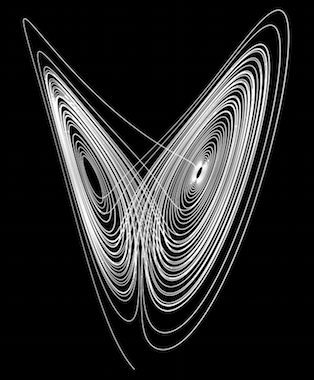
\includegraphics[scale = 0.6]{images/lorenz2.png}
\caption{Plot of the Lorenz strange attractor for $\sigma$ = 10, $\rho$ = 28, and $\beta$ = 8/3 \cite{bourke}}
\label{fig:lorenz}
\end{figure}


%%%%%%%%%%%%%%%%%%%%%%%%%%%%%%%%%%%%%%%%%%%%%%%%%%%%%%
%\vspace{-10pt}
\section{Methods}
\label{sec:methods}

Three simulations were conducted in $\Matlab$ to gain a better understanding of how the Lorenz system evolves.  Data was acquired using a simulation of the Lorenz system which gave three vectors representing the x-, y-, and z-coordinates of the system as it evolved. 

For the first simulation, data was used solely from the X vector (the position of the Lorenz system projected onto the x axis). By running the simulation of the Lorenz system repeatedly, a matrix was constructed by concatenating the X vectors togethers for different values of $\beta$, ranging from 1 to 10.  From this matrix, the sensitivity of various functions to changes in $\beta$ was calculated using the following equation:

\begin{equation}
	Sensitivity = \frac{dE[f(x)]}{d\beta}
\end{equation}

\noindent Thus, to calculate the sensitivity of a given function to $\beta$, the X vector was divided into sections and the value of the function for each section was calculated.  Then, based on the value of the function for each section, the expectation of that function for the entire X vector was calculated.  Finally, the change in this expectation value over the change in $\beta$ for small changes in $\beta$ was plotted to observe the sensitivity over a range of values.  This process was completed both for the fourth central moment (figure~\ref{fig:4thX}) and the sixth central moment (figure~\ref{fig:6thX}).

Next, the evolution of the R vector was examined, where $R = \sqrt{X^2 + Y^2 + Z^2}$ (figure~\ref{fig:REvolution}). This was to ensure that no large jumps were occurring in the evolution of the R vector due to the step size being used.  In addition, the sensitivity of the fourth and sixth central moment were plotted again, this time using the R vector (figures \ref{fig:4thR} and \ref{fig:6thR} respectively).

Finally, using the pcolor plotting tool in \Matlab, the Fast Fourier Transform of the X vector multiplied by a Hamming window was plotted against different values of $\beta$.  In the resulting plots, the color of the plot represents the intensity of the FFT at a specific value of $\beta$ and frequency.  Figure \ref{fig:pcolor1} shows this plot for values of $\beta$ from 0 to 100 while figure \ref{fig:pcolor2} examines values from 0 to 10.  Lastly, figure \ref{fig:pcolor3} is a closer look at how the frequencies transition in figure \ref{fig:pcolor2}.


%%%%%%%%%%%%%%%%%%%%%%%%%%%%%%%%%%%%%%%%%%%%%%%%%%%%%%
%\vspace{-10pt}
\section{Results}
\label{sec:results}

\begin{figure}[H]
\centering
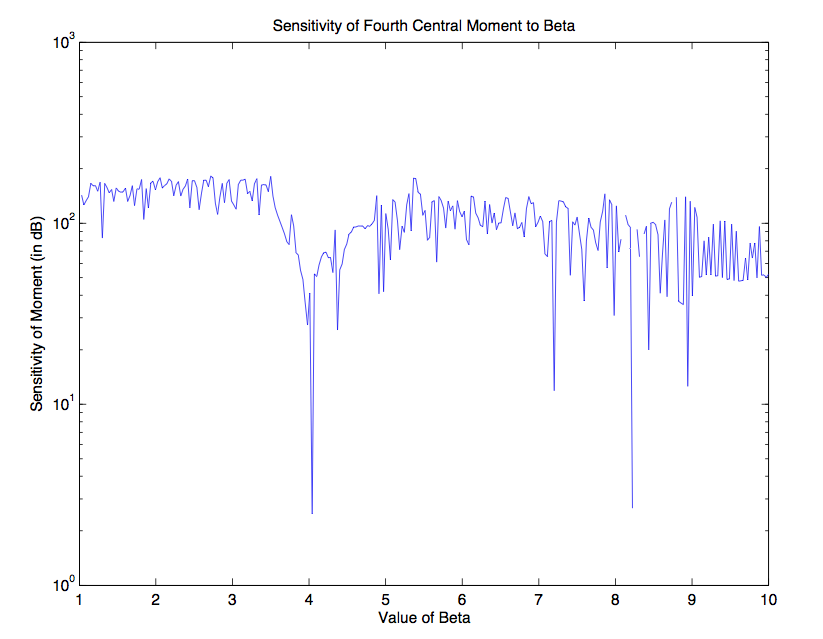
\includegraphics[totalheight=0.4\textheight]{images/SensitivityFourth.png}
\caption{4th central moment sensitivity using X vector}
\label{fig:4thX}
\end{figure}
\begin{figure}[H]
\centering
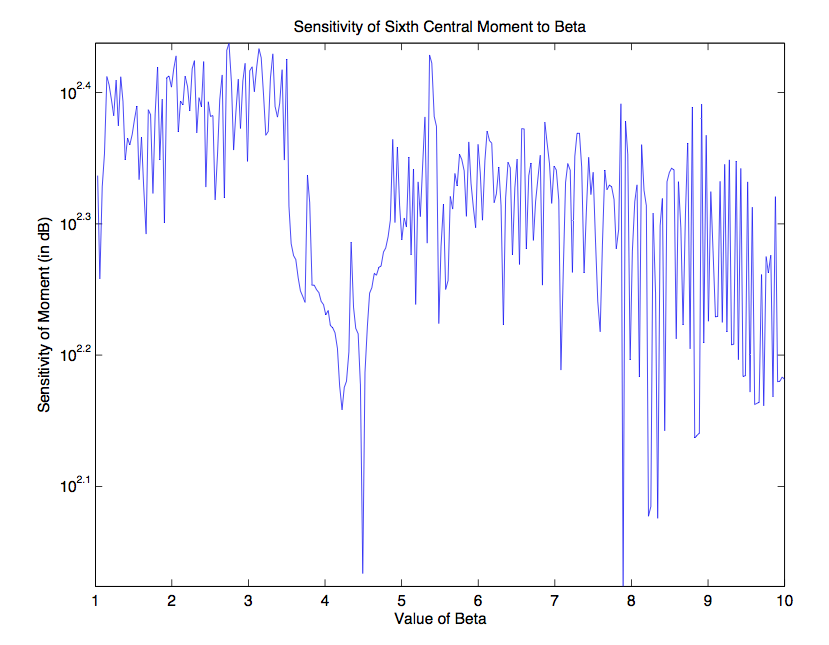
\includegraphics[totalheight=0.4\textheight]{images/SensitivitySixth.png}
\caption{6th central moment sensitivity using X vector}
\label{fig:6thX}
\end{figure}
\begin{figure}[H]
\centering
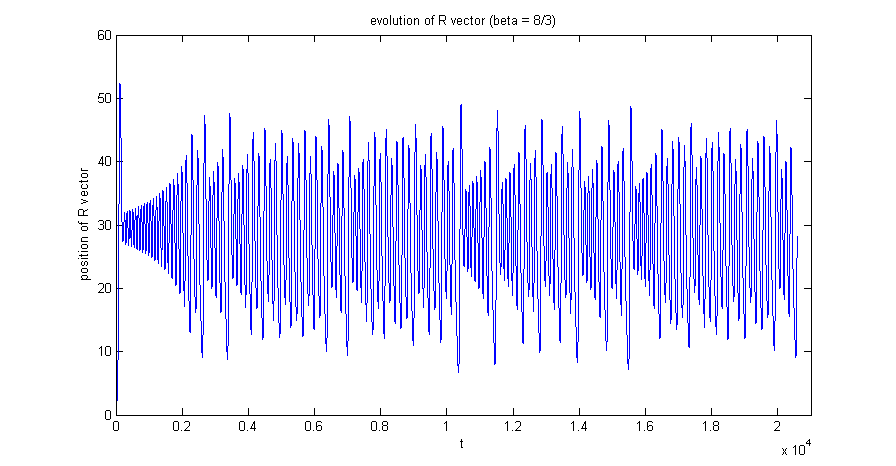
\includegraphics[scale = 0.6]{images/REvolution.png}
\caption{Evolution of R vector for $\beta = 8/3$}
\label{fig:REvolution}
\end{figure}
\begin{figure}[H]
\centering
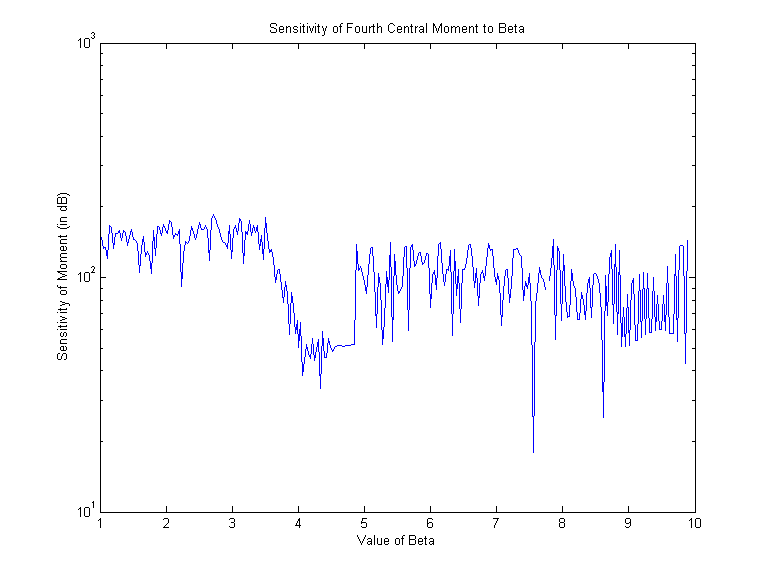
\includegraphics[scale = 0.6]{images/RSensitivityFourth.png}
\caption{4th central moment sensitivity using R vector}
\label{fig:4thR}
\end{figure}
\begin{figure}[H]
\centering
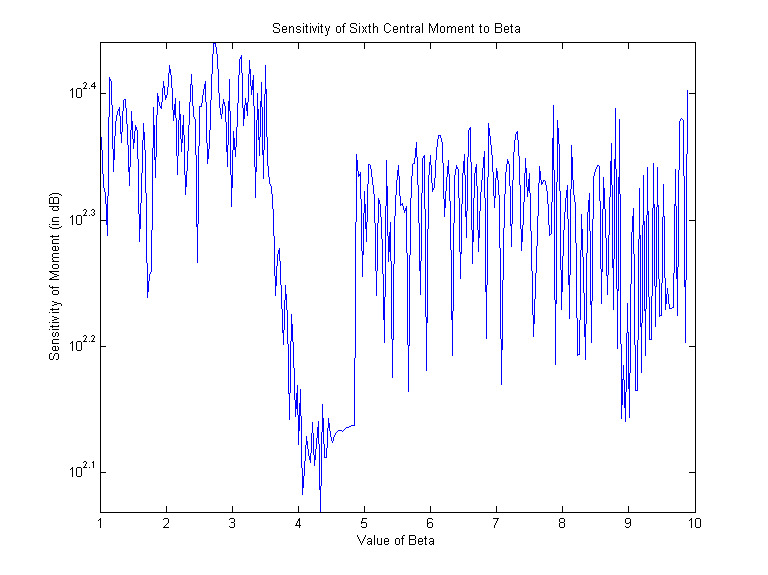
\includegraphics[scale = 0.6]{images/RSensitivitySixth.png}
\caption{6th central moment sensitivity using R vector}
\label{fig:6thR}
\end{figure}
\begin{figure}[H]
\centering
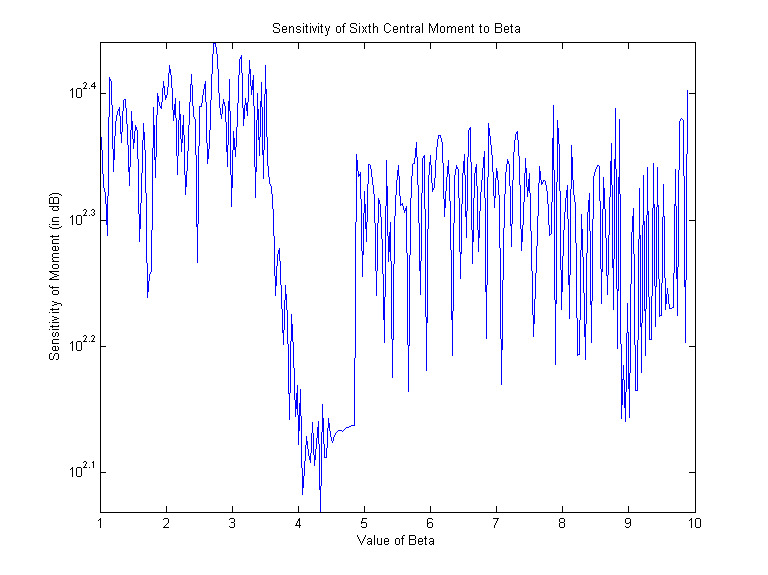
\includegraphics[scale = 0.6]{images/RSensitivitySixth.png}
\caption{6th central moment sensitivity using R vector}
\label{fig:6thR}
\end{figure}
\begin{figure}[H]
\centering
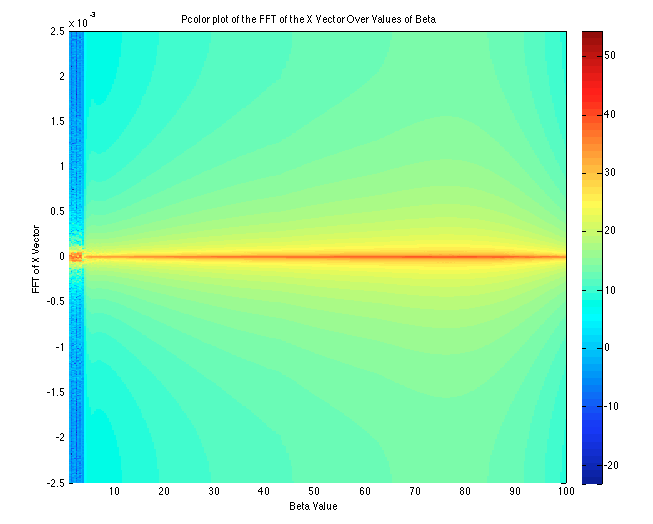
\includegraphics[totalheight=0.4\textheight]{images/pcolor1.png}
\caption{Pcolor plot of the FFT of the X Vector over value of $\beta$ from 0 to 100}
\label{fig:pcolor1}
\end{figure}
\begin{figure}[H]
\centering
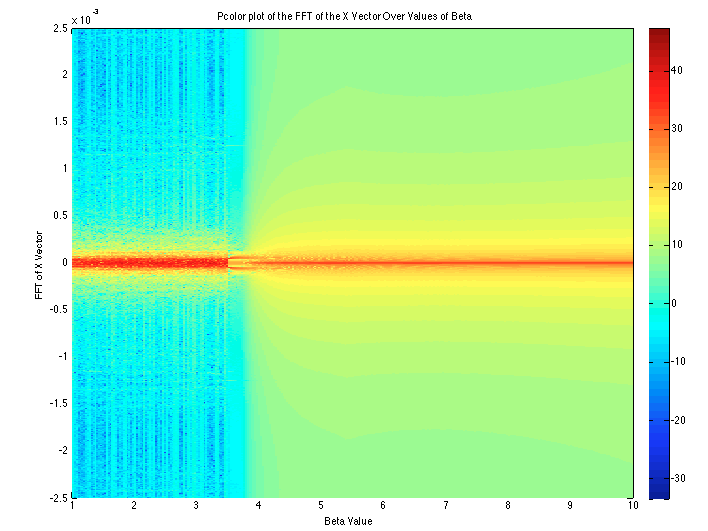
\includegraphics[totalheight=0.4\textheight]{images/pcolor2.png}
\caption{Pcolor plot of the FFT of the X Vector over value of $\beta$ from 0 to 10}
\label{fig:pcolor2}
\end{figure}
\begin{figure}[H]
\centering
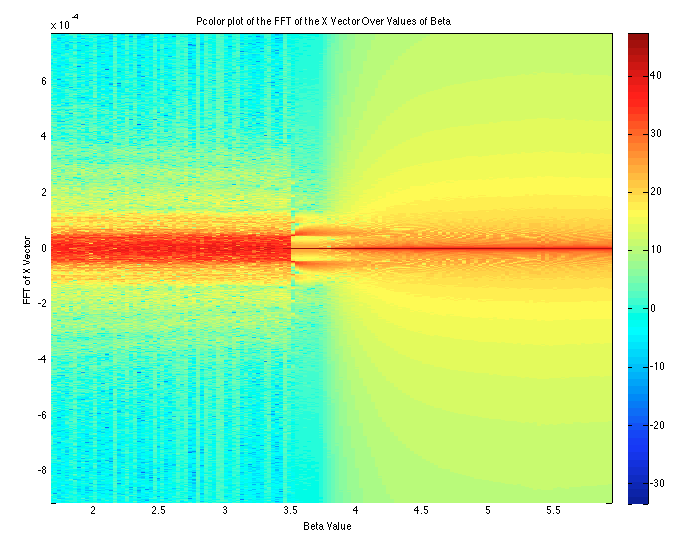
\includegraphics[totalheight=0.4\textheight]{images/pcolor3.png}
\caption{A closer look at figure \ref{fig:pcolor2} showing a bifurcation that occurs in the system}
\label{fig:pcolor3}
\end{figure}
%pcolor plot here

%\vspace{-10pt}
\section{Conclusions}
\label{sec:conclusion}
Several observations can be made from the three simulations conducted in this work.  First, the X vector of the Lorenz system appears to be very sensitive to the fourth and sixth central moment, and when $\beta$ was allowed to vary from 1 to 100, the sensitivity appeared to go up without bound as $\beta$ approached 100.  The second two simulations were conducted to examine if this occurred due to the step size of the system or due to some particular value of $\beta$.  By plotting the evolution of the magnitude of the R vector over time, it was confirmed that the system was not making an unusually large jumps due to the step size, and thus, this was likely not a cause of the large increase in sensitivity.  When the the FFT of the X vector was plotted against $\beta$, it was shown that the system changed very little for $\beta$ values above 5.  This likely meant that large sensitivity values obtained for values of $\beta$ greater than 10 were more a result of how the system evolved rather than any particular function.  As a result all plots were redone for $\beta$ ranging between 1 and 10.  The system was still sensitive to the fourth and sixth central moment, but in a more reasonable manner.  In addition, by examining the color plot around values of $\beta$ between 3.5 and 4.5 some bifurcation behaviors were observed.  Based on this work, the Lorenz system is fairly sensitive to the fourth and sixth central moments, and the relationship between the system and these two functions deserves further investigation.

\section{Acknowledgements}
\label{sec:Ack}
We would like to acknowledge Moiseev Igor for the open source \Matlab \ Lorenz system generator.


%Bibliography
\bibliographystyle{IEEEtran}
\bibliography{proposal_refs.bib}

\end{document}